%%%% PROCESAR con PdfLaTeX !!!!!


\documentclass[12pt]{book}
\usepackage{geometry}\geometry{top=2cm,bottom=2cm,left=3cm,right=3cm}
\usepackage{amssymb}
\usepackage{amsmath}
\usepackage{graphicx}
\usepackage{txfonts}
%\usepackage{hyperref}
\usepackage[hidelinks]{hyperref}
\usepackage[spanish]{babel}
\setcounter{tocdepth}{3}
\usepackage[usenames]{color}

\usepackage[hidelinks]{hyperref}
\hypersetup{
    colorlinks=true,
    linkcolor=black,
    filecolor=magenta,      
    urlcolor=cyan,
    pdftitle={Sharelatex Example},
    bookmarks=true,
%    pdfpagemode=FullScreen,
}


\begin{document}
\thispagestyle{empty}

\begin {center}

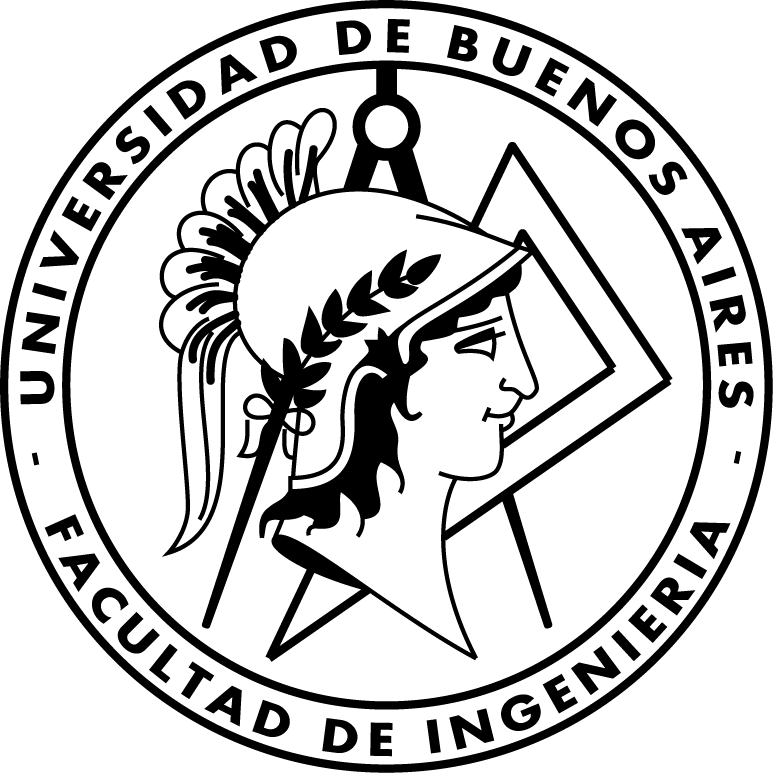
\includegraphics[scale=.4]{Logo-fiuba_big.png}

\medskip
UNIVERSIDAD DE BUENOS AIRES

Facultad de Ingenier\'ia

Departamento de Computaci\'on


\vspace{3cm}


\textbf{\large Algoritmos y complejidad computacional}

\vspace{2cm}


Este es un modesto aporte para los alumnos de la f\'acultad de ingenier\'ia  de la UBA de las carreras de licenciatura en an\'alsis de sistemas e ingenier\'ia inform\'atica.
De ninguna man\'era pretende ser una gu\'ia de estudio, ni remplaza las clases presenciales, el material oficial de la catedra esta disponible en el web site de la m\'ateria.
\\
\url{http://materias.fi.uba.ar/7510/}

\end {center}


\vspace{2.5cm}

\noindent Autor:\,	Isaac Edgar Camacho Ocampo
 
\noindent Carrera:\,	Licenciatura en An\'alisis de sistemas

\vspace{1cm}

\vspace{1cm}

\noindent Buenos Aires, 2019

\newpage


\tableofcontents
\chapter*{Abstract} % si no queremos que añada la palabra "Capitulo"
\addcontentsline{toc}{section}{Resumen} % si queremos que aparezca en el índice
\markboth{Abstract}{Abstract} % encabezado
\section{¿Qué es un algoritmo?}
Podemos decir que es la especificación de una secuencia de instrucciones para a partir de datos de entrada resolver un problema con un mecanismo automáticos es decir resolver un problema tomando tus entradas y entregando datos de salida o resultados la especificación puede ser de diversas maneras en lenguaje natural en pseudocódigo etcétera
Pero esencialmente siempre se llega a que la especificación es que hay que hacer a partir de los datos de entrada para obtener los datos de salida

\section{¿Qué es un buen algoritmo?}
la primera idea que tenemos es que un algoritmo funciona cuando resuelve el problema en cuestión, bueno ahora supongamos que funciona el algoritmo qué criterios debemos tomar para decir que un algoritmo es bueno, podemos ir con algoritmos bueno cuando es claro es decir fácil entendible, o cuando es fácil de implementar o qué es un buen algoritmo cuando es eficiente o cuando es rápido todos estos criterios son válidos el más popular para determinar la calidad de un algoritmo es el tiempo es decir un algoritmo es bueno cuando funciona rápidamente

Dados algoritmos que resuelven un mismo problema ? ¿Cuál es mejor?
Según el criterio del tiempo podemos decir que es mejor el que funciona más rápido, evidentemente en la actualidad es preferible un algoritmo que resolver rápidamente un problema a otro que lo hace en más tiempo

\section{¿Cuando un problema está bien resuelto?}
Bueno esencialmente un problema está bien resultó cuando el algoritmo es bueno es decir cuando el algoritmo es aceptable según los criterios que hayamos seleccionado generalmente en nuestros problemas de grafos el tiempo es el factor decisivo.

\section{Repaso - Complejidad computacional}
El objetivo es querer medir el tiempo de ejecución de los algoritmos queremos saber cuánto tarda en función de los datos de entrada.
Mesa virtual utilizar una forma de medir el tiempo de ejecución de un algoritmo utilizando el peor caso en función del tamaño de la entrada del algoritmo

Para una entrada de tamaño n que es lo peor que le puede pasar es decir para una entrada genérica el peor caso posible

Y cómo medimos el tamaño de la entrada del algoritmo
Para esto y dos posibilidades

\subsubsection{Modelo uniforme}
Asumimos que cada dato individual es decir un entero o un booleano ocupa una posición individual de memoria por ejemplo decimos que un arreglo de n elementos tiene tamaño n

En el siguiente ejemplo podemos ver un algoritmo para determinar si un número ingresado por parámetro es primo un error muy común consiste en creer que el tamaño de la entrada es el parámetro de entrada sin embargo podemos ver que para este algoritmo el parámetro de entrada es el número a calcular y el tamaño de la entrada también es uno

Uno estaría tentado a decir que función de complejidad de algoritmos sería o dn pero podemos ver que el tamaño de la entrada es 1

Pero podemos ver que si el número es lo suficientemente grande este algoritmo tardará mucho y su función de complejidad no será o dn

\subsubsection{Modelo logarítmico}
Se mide el tamaño en bits de cada dato individual por ejemplo el tamaño de un entero k se define como n igual a logaritmo en base 2 de ca más uno y tomar la parte entera

Podemos darnos cuentas que este algoritmo es malo porque para números grandes lo peor que le puede pasar es que recorra todos los números intermedios y después de un cálculo minucioso 
podemos determinar que el orden de complejidad de este algoritmo es de 2 a la n
El orden de complejidad es exponencial respecto de la cantidad de bits que ocupa el número




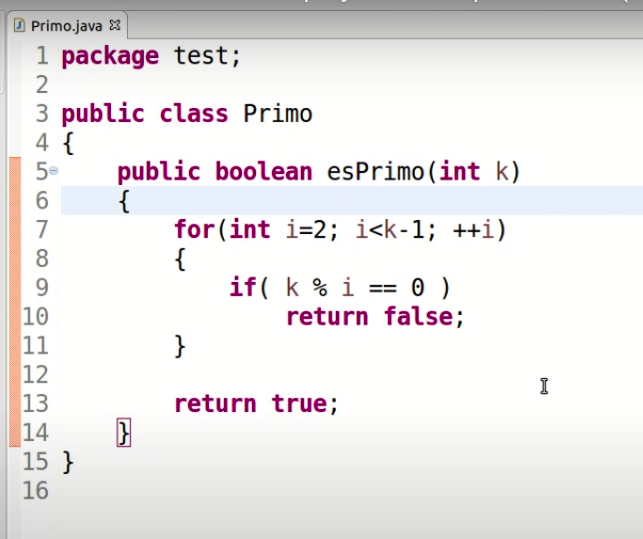
\includegraphics[scale=.4]{./image/primo.png}



\chapter{Algoritmos dividir y conquistar}
\section{Conocimientos previos}
\section{Estado del arte}
\chapter{Grafos algoritmos sobre grafos}
\section{Teoría clásica}
\subsection{Definición de variables}
\subsection{Pruebas y refutaciones}
\section{Hipótesis}
\chapter{Problema de árbol generador mínimo}
\section{Simulación de resultados}
\subsection{Suposiciones}
\subsection{Modelos}
\section{Resultados preliminares}
\section{Resultados postprocesados}
\subsection{Valores atípicos}
\subsection{Correlaciones}
\chapter{Problema de flujo máximo}
\chapter{Problema de camino mínimo}
\chapter{Algoritmos de fuerza bruta y backtracking}
\chapter{Problemas NP completos}
\chapter{Heurísticas y algoritmos golosos}

\chapter{Algoritmos genéticos}
\chapter{Algoritmos evolutivos}
\end{document}


